\documentclass[1p]{elsarticle_modified}
%\bibliographystyle{elsarticle-num}

%\usepackage[colorlinks]{hyperref}
%\usepackage{abbrmath_seonhwa} %\Abb, \Ascr, \Acal ,\Abf, \Afrak
\usepackage{amsfonts}
\usepackage{amssymb}
\usepackage{amsmath}
\usepackage{amsthm}
\usepackage{scalefnt}
\usepackage{amsbsy}
\usepackage{kotex}
\usepackage{caption}
\usepackage{subfig}
\usepackage{color}
\usepackage{graphicx}
\usepackage{xcolor} %% white, black, red, green, blue, cyan, magenta, yellow
\usepackage{float}
\usepackage{setspace}
\usepackage{hyperref}

\usepackage{tikz}
\usetikzlibrary{arrows}

\usepackage{multirow}
\usepackage{array} % fixed length table
\usepackage{hhline}

%%%%%%%%%%%%%%%%%%%%%
\makeatletter
\renewcommand*\env@matrix[1][\arraystretch]{%
	\edef\arraystretch{#1}%
	\hskip -\arraycolsep
	\let\@ifnextchar\new@ifnextchar
	\array{*\c@MaxMatrixCols c}}
\makeatother %https://tex.stackexchange.com/questions/14071/how-can-i-increase-the-line-spacing-in-a-matrix
%%%%%%%%%%%%%%%

\usepackage[normalem]{ulem}

\newcommand{\msout}[1]{\ifmmode\text{\sout{\ensuremath{#1}}}\else\sout{#1}\fi}
%SOURCE: \msout is \stkout macro in https://tex.stackexchange.com/questions/20609/strikeout-in-math-mode

\newcommand{\cancel}[1]{
	\ifmmode
	{\color{red}\msout{#1}}
	\else
	{\color{red}\sout{#1}}
	\fi
}

\newcommand{\add}[1]{
	{\color{blue}\uwave{#1}}
}

\newcommand{\replace}[2]{
	\ifmmode
	{\color{red}\msout{#1}}{\color{blue}\uwave{#2}}
	\else
	{\color{red}\sout{#1}}{\color{blue}\uwave{#2}}
	\fi
}

\newcommand{\Sol}{\mathcal{S}} %segment
\newcommand{\D}{D} %diagram
\newcommand{\A}{\mathcal{A}} %arc


%%%%%%%%%%%%%%%%%%%%%%%%%%%%%5 test

\def\sl{\operatorname{\textup{SL}}(2,\Cbb)}
\def\psl{\operatorname{\textup{PSL}}(2,\Cbb)}
\def\quan{\mkern 1mu \triangleright \mkern 1mu}

\theoremstyle{definition}
\newtheorem{thm}{Theorem}[section]
\newtheorem{prop}[thm]{Proposition}
\newtheorem{lem}[thm]{Lemma}
\newtheorem{ques}[thm]{Question}
\newtheorem{cor}[thm]{Corollary}
\newtheorem{defn}[thm]{Definition}
\newtheorem{exam}[thm]{Example}
\newtheorem{rmk}[thm]{Remark}
\newtheorem{alg}[thm]{Algorithm}

\newcommand{\I}{\sqrt{-1}}
\begin{document}

%\begin{frontmatter}
%
%\title{Boundary parabolic representations of knots up to 8 crossings}
%
%%% Group authors per affiliation:
%\author{Yunhi Cho} 
%\address{Department of Mathematics, University of Seoul, Seoul, Korea}
%\ead{yhcho@uos.ac.kr}
%
%
%\author{Seonhwa Kim} %\fnref{s_kim}}
%\address{Center for Geometry and Physics, Institute for Basic Science, Pohang, 37673, Korea}
%\ead{ryeona17@ibs.re.kr}
%
%\author{Hyuk Kim}
%\address{Department of Mathematical Sciences, Seoul National University, Seoul 08826, Korea}
%\ead{hyukkim@snu.ac.kr}
%
%\author{Seokbeom Yoon}
%\address{Department of Mathematical Sciences, Seoul National University, Seoul, 08826,  Korea}
%\ead{sbyoon15@snu.ac.kr}
%
%\begin{abstract}
%We find all boundary parabolic representation of knots up to 8 crossings.
%
%\end{abstract}
%\begin{keyword}
%    \MSC[2010] 57M25 
%\end{keyword}
%
%\end{frontmatter}

%\linenumbers
%\tableofcontents
%
\newcommand\colored[1]{\textcolor{white}{\rule[-0.35ex]{0.8em}{1.4ex}}\kern-0.8em\color{red} #1}%
%\newcommand\colored[1]{\textcolor{white}{ #1}\kern-2.17ex	\textcolor{white}{ #1}\kern-1.81ex	\textcolor{white}{ #1}\kern-2.15ex\color{red}#1	}

{\Large $\underline{12n_{0539}~(K12n_{0539})}$}

\setlength{\tabcolsep}{10pt}
\renewcommand{\arraystretch}{1.6}
\vspace{1cm}\begin{tabular}{m{100pt}>{\centering\arraybackslash}m{274pt}}
\multirow{5}{120pt}{
	\centering
	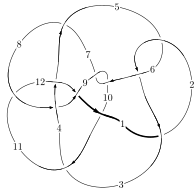
\includegraphics[width=112pt]{../../../GIT/diagram.site/Diagrams/png/2628_12n_0539.png}\\
\ \ \ A knot diagram\footnotemark}&
\allowdisplaybreaks
\textbf{Linearized knot diagam} \\
\cline{2-2}
 &
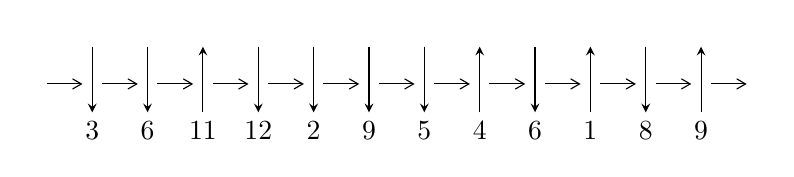
\begin{tikzpicture}[x=20pt, y=17pt]
	% nodes
	\node (C0) at (0, 0) {};
	\node (C1) at (1, 0) {};
	\node (C1U) at (1, +1) {};
	\node (C1D) at (1, -1) {3};

	\node (C2) at (2, 0) {};
	\node (C2U) at (2, +1) {};
	\node (C2D) at (2, -1) {6};

	\node (C3) at (3, 0) {};
	\node (C3U) at (3, +1) {};
	\node (C3D) at (3, -1) {11};

	\node (C4) at (4, 0) {};
	\node (C4U) at (4, +1) {};
	\node (C4D) at (4, -1) {12};

	\node (C5) at (5, 0) {};
	\node (C5U) at (5, +1) {};
	\node (C5D) at (5, -1) {2};

	\node (C6) at (6, 0) {};
	\node (C6U) at (6, +1) {};
	\node (C6D) at (6, -1) {9};

	\node (C7) at (7, 0) {};
	\node (C7U) at (7, +1) {};
	\node (C7D) at (7, -1) {5};

	\node (C8) at (8, 0) {};
	\node (C8U) at (8, +1) {};
	\node (C8D) at (8, -1) {4};

	\node (C9) at (9, 0) {};
	\node (C9U) at (9, +1) {};
	\node (C9D) at (9, -1) {6};

	\node (C10) at (10, 0) {};
	\node (C10U) at (10, +1) {};
	\node (C10D) at (10, -1) {1};

	\node (C11) at (11, 0) {};
	\node (C11U) at (11, +1) {};
	\node (C11D) at (11, -1) {8};

	\node (C12) at (12, 0) {};
	\node (C12U) at (12, +1) {};
	\node (C12D) at (12, -1) {9};
	\node (C13) at (13, 0) {};

	% arrows
	\draw[->,>={angle 60}]
	(C0) edge (C1) (C1) edge (C2) (C2) edge (C3) (C3) edge (C4) (C4) edge (C5) (C5) edge (C6) (C6) edge (C7) (C7) edge (C8) (C8) edge (C9) (C9) edge (C10) (C10) edge (C11) (C11) edge (C12) (C12) edge (C13) ;	\draw[->,>=stealth]
	(C1U) edge (C1D) (C2U) edge (C2D) (C3D) edge (C3U) (C4U) edge (C4D) (C5U) edge (C5D) (C6U) edge (C6D) (C7U) edge (C7D) (C8D) edge (C8U) (C9U) edge (C9D) (C10D) edge (C10U) (C11U) edge (C11D) (C12D) edge (C12U) ;
	\end{tikzpicture} \\
\hhline{~~} \\& 
\textbf{Solving Sequence} \\ \cline{2-2} 
 &
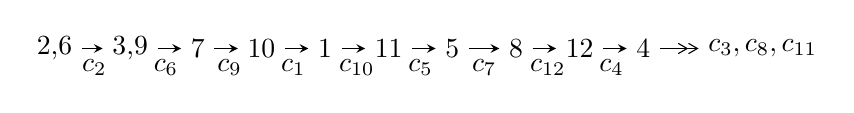
\begin{tikzpicture}[x=23pt, y=7pt]
	% node
	\node (A0) at (-1/8, 0) {2,6};
	\node (A1) at (17/16, 0) {3,9};
	\node (A2) at (17/8, 0) {7};
	\node (A3) at (25/8, 0) {10};
	\node (A4) at (33/8, 0) {1};
	\node (A5) at (41/8, 0) {11};
	\node (A6) at (49/8, 0) {5};
	\node (A7) at (57/8, 0) {8};
	\node (A8) at (65/8, 0) {12};
	\node (A9) at (73/8, 0) {4};
	\node (C1) at (1/2, -1) {$c_{2}$};
	\node (C2) at (13/8, -1) {$c_{6}$};
	\node (C3) at (21/8, -1) {$c_{9}$};
	\node (C4) at (29/8, -1) {$c_{1}$};
	\node (C5) at (37/8, -1) {$c_{10}$};
	\node (C6) at (45/8, -1) {$c_{5}$};
	\node (C7) at (53/8, -1) {$c_{7}$};
	\node (C8) at (61/8, -1) {$c_{12}$};
	\node (C9) at (69/8, -1) {$c_{4}$};
	\node (A10) at (11, 0) {$c_{3},c_{8},c_{11}$};

	% edge
	\draw[->,>=stealth]	
	(A0) edge (A1) (A1) edge (A2) (A2) edge (A3) (A3) edge (A4) (A4) edge (A5) (A5) edge (A6) (A6) edge (A7) (A7) edge (A8) (A8) edge (A9) ;
	\draw[->>,>={angle 60}]	
	(A9) edge (A10);
\end{tikzpicture} \\ 

\end{tabular} \\

\footnotetext{
The image of knot diagram is generated by the software ``\textbf{Draw programme}" developed by Andrew Bartholomew(\url{http://www.layer8.co.uk/maths/draw/index.htm\#Running-draw}), where we modified some parts for our purpose(\url{https://github.com/CATsTAILs/LinksPainter}).
}\phantom \\ \newline 
\centering \textbf{Ideals for irreducible components\footnotemark of $X_{\text{par}}$} 
 
\begin{align*}
I^u_{1}&=\langle 
1.71224\times10^{120} u^{84}+1.40203\times10^{120} u^{83}+\cdots+3.73013\times10^{118} b-2.07454\times10^{120},\\
\phantom{I^u_{1}}&\phantom{= \langle  }8.58971\times10^{120} u^{84}+5.94299\times10^{120} u^{83}+\cdots+4.10314\times10^{119} a-4.74408\times10^{120},\\
\phantom{I^u_{1}}&\phantom{= \langle  }u^{85}-24 u^{83}+\cdots+10 u+1\rangle \\
I^u_{2}&=\langle 
-10 u^{21}+53 u^{19}+\cdots+b-15,\;-10 u^{21}+54 u^{19}+\cdots+a-13,\;u^{22}+u^{21}+\cdots-2 u+1\rangle \\
\\
\end{align*}
\raggedright * 2 irreducible components of $\dim_{\mathbb{C}}=0$, with total 107 representations.\\
\footnotetext{All coefficients of polynomials are rational numbers. But the coefficients are sometimes approximated in decimal forms when there is not enough margin.}
\newpage
\renewcommand{\arraystretch}{1}
\centering \section*{I. $I^u_{1}= \langle 1.71\times10^{120} u^{84}+1.40\times10^{120} u^{83}+\cdots+3.73\times10^{118} b-2.07\times10^{120},\;8.59\times10^{120} u^{84}+5.94\times10^{120} u^{83}+\cdots+4.10\times10^{119} a-4.74\times10^{120},\;u^{85}-24 u^{83}+\cdots+10 u+1 \rangle$}
\flushleft \textbf{(i) Arc colorings}\\
\begin{tabular}{m{7pt} m{180pt} m{7pt} m{180pt} }
\flushright $a_{2}=$&$\begin{pmatrix}1\\0\end{pmatrix}$ \\
\flushright $a_{6}=$&$\begin{pmatrix}0\\u\end{pmatrix}$ \\
\flushright $a_{3}=$&$\begin{pmatrix}1\\u^2\end{pmatrix}$ \\
\flushright $a_{9}=$&$\begin{pmatrix}-20.9345 u^{84}-14.4840 u^{83}+\cdots+267.776 u+11.5621\\-45.9029 u^{84}-37.5866 u^{83}+\cdots+629.922 u+55.6158\end{pmatrix}$ \\
\flushright $a_{7}=$&$\begin{pmatrix}11.1468 u^{84}+8.19621 u^{83}+\cdots-72.3417 u+9.67525\\18.6966 u^{84}+17.0401 u^{83}+\cdots-217.270 u-19.2457\end{pmatrix}$ \\
\flushright $a_{10}=$&$\begin{pmatrix}-20.9345 u^{84}-14.4840 u^{83}+\cdots+267.776 u+11.5621\\-57.1007 u^{84}-46.1321 u^{83}+\cdots+795.697 u+70.0998\end{pmatrix}$ \\
\flushright $a_{1}=$&$\begin{pmatrix}- u^2+1\\- u^4\end{pmatrix}$ \\
\flushright $a_{11}=$&$\begin{pmatrix}-30.8822 u^{84}-22.1361 u^{83}+\cdots+408.995 u+23.4304\\-46.8081 u^{84}-37.9200 u^{83}+\cdots+649.457 u+57.1070\end{pmatrix}$ \\
\flushright $a_{5}=$&$\begin{pmatrix}u\\u\end{pmatrix}$ \\
\flushright $a_{8}=$&$\begin{pmatrix}3.64203 u^{84}+1.55727 u^{83}+\cdots+23.6473 u+18.5192\\11.1918 u^{84}+10.4012 u^{83}+\cdots-121.281 u-10.4017\end{pmatrix}$ \\
\flushright $a_{12}=$&$\begin{pmatrix}-8.59326 u^{84}-8.98215 u^{83}+\cdots+100.400 u+15.7211\\-34.9414 u^{84}-30.6980 u^{83}+\cdots+434.117 u+39.2473\end{pmatrix}$ \\
\flushright $a_{4}=$&$\begin{pmatrix}13.6180 u^{84}+13.8934 u^{83}+\cdots-145.844 u-18.0597\\48.0968 u^{84}+41.5976 u^{83}+\cdots-603.928 u-54.4575\end{pmatrix}$\\&\end{tabular}
\flushleft \textbf{(ii) Obstruction class $= -1$}\\~\\
\flushleft \textbf{(iii) Cusp Shapes $= 171.919 u^{84}+151.328 u^{83}+\cdots-2175.77 u-192.981$}\\~\\
\newpage\renewcommand{\arraystretch}{1}
\flushleft \textbf{(iv) u-Polynomials at the component}\newline \\
\begin{tabular}{m{50pt}|m{274pt}}
Crossings & \hspace{64pt}u-Polynomials at each crossing \\
\hline $$\begin{aligned}c_{1}\end{aligned}$$&$\begin{aligned}
&u^{85}+48 u^{84}+\cdots+76 u+1
\end{aligned}$\\
\hline $$\begin{aligned}c_{2},c_{5}\end{aligned}$$&$\begin{aligned}
&u^{85}-24 u^{83}+\cdots+10 u-1
\end{aligned}$\\
\hline $$\begin{aligned}c_{3}\end{aligned}$$&$\begin{aligned}
&u^{85}-22 u^{83}+\cdots-68443 u-15487
\end{aligned}$\\
\hline $$\begin{aligned}c_{4}\end{aligned}$$&$\begin{aligned}
&u^{85}+3 u^{84}+\cdots-115 u+29
\end{aligned}$\\
\hline $$\begin{aligned}c_{6},c_{9}\end{aligned}$$&$\begin{aligned}
&u^{85}+8 u^{84}+\cdots+33526 u+4031
\end{aligned}$\\
\hline $$\begin{aligned}c_{7}\end{aligned}$$&$\begin{aligned}
&u^{85}-8 u^{84}+\cdots-747 u-17
\end{aligned}$\\
\hline $$\begin{aligned}c_{8}\end{aligned}$$&$\begin{aligned}
&u^{85}-3 u^{84}+\cdots-24 u+11
\end{aligned}$\\
\hline $$\begin{aligned}c_{10}\end{aligned}$$&$\begin{aligned}
&u^{85}+u^{84}+\cdots-653233343 u-56357257
\end{aligned}$\\
\hline $$\begin{aligned}c_{11}\end{aligned}$$&$\begin{aligned}
&u^{85}+6 u^{84}+\cdots-17 u+1
\end{aligned}$\\
\hline $$\begin{aligned}c_{12}\end{aligned}$$&$\begin{aligned}
&u^{85}+u^{84}+\cdots-7039 u-223
\end{aligned}$\\
\hline
\end{tabular}\\~\\
\newpage\renewcommand{\arraystretch}{1}
\flushleft \textbf{(v) Riley Polynomials at the component}\newline \\
\begin{tabular}{m{50pt}|m{274pt}}
Crossings & \hspace{64pt}Riley Polynomials at each crossing \\
\hline $$\begin{aligned}c_{1}\end{aligned}$$&$\begin{aligned}
&y^{85}-16 y^{84}+\cdots+5764 y-1
\end{aligned}$\\
\hline $$\begin{aligned}c_{2},c_{5}\end{aligned}$$&$\begin{aligned}
&y^{85}-48 y^{84}+\cdots+76 y-1
\end{aligned}$\\
\hline $$\begin{aligned}c_{3}\end{aligned}$$&$\begin{aligned}
&y^{85}-44 y^{84}+\cdots+7600305635 y-239847169
\end{aligned}$\\
\hline $$\begin{aligned}c_{4}\end{aligned}$$&$\begin{aligned}
&y^{85}-13 y^{84}+\cdots+50693 y-841
\end{aligned}$\\
\hline $$\begin{aligned}c_{6},c_{9}\end{aligned}$$&$\begin{aligned}
&y^{85}-84 y^{84}+\cdots+4537701460 y-16248961
\end{aligned}$\\
\hline $$\begin{aligned}c_{7}\end{aligned}$$&$\begin{aligned}
&y^{85}-40 y^{84}+\cdots+290429 y-289
\end{aligned}$\\
\hline $$\begin{aligned}c_{8}\end{aligned}$$&$\begin{aligned}
&y^{85}-13 y^{84}+\cdots+6208 y-121
\end{aligned}$\\
\hline $$\begin{aligned}c_{10}\end{aligned}$$&$\begin{aligned}
&y^{85}+53 y^{84}+\cdots+392522021882255677 y-3176140416564049
\end{aligned}$\\
\hline $$\begin{aligned}c_{11}\end{aligned}$$&$\begin{aligned}
&y^{85}+8 y^{84}+\cdots+23 y-1
\end{aligned}$\\
\hline $$\begin{aligned}c_{12}\end{aligned}$$&$\begin{aligned}
&y^{85}+25 y^{84}+\cdots+6405495 y-49729
\end{aligned}$\\
\hline
\end{tabular}\\~\\
\newpage\flushleft \textbf{(vi) Complex Volumes and Cusp Shapes}
$$\begin{array}{c|c|c}  
\text{Solutions to }I^u_{1}& \I (\text{vol} + \sqrt{-1}CS) & \text{Cusp shape}\\
 \hline 
\begin{aligned}
u &= \phantom{-}0.005353 + 1.000360 I \\
a &= \phantom{-}0.18285 - 1.48764 I \\
b &= \phantom{-}0.349188 - 0.373795 I\end{aligned}
 & -1.93409 + 0.60336 I & \phantom{-0.000000 } 0 \\ \hline\begin{aligned}
u &= \phantom{-}0.005353 - 1.000360 I \\
a &= \phantom{-}0.18285 + 1.48764 I \\
b &= \phantom{-}0.349188 + 0.373795 I\end{aligned}
 & -1.93409 - 0.60336 I & \phantom{-0.000000 } 0 \\ \hline\begin{aligned}
u &= \phantom{-}0.188620 + 0.969304 I \\
a &= \phantom{-}0.19737 + 1.77663 I \\
b &= -0.062291 + 0.128491 I\end{aligned}
 & -1.46515 + 11.85320 I & \phantom{-0.000000 } 0 \\ \hline\begin{aligned}
u &= \phantom{-}0.188620 - 0.969304 I \\
a &= \phantom{-}0.19737 - 1.77663 I \\
b &= -0.062291 - 0.128491 I\end{aligned}
 & -1.46515 - 11.85320 I & \phantom{-0.000000 } 0 \\ \hline\begin{aligned}
u &= -0.840878 + 0.483325 I \\
a &= \phantom{-}0.501916 - 1.283270 I \\
b &= \phantom{-}1.34341 - 1.06918 I\end{aligned}
 & \phantom{-}3.51388 - 1.61241 I & \phantom{-0.000000 } 0 \\ \hline\begin{aligned}
u &= -0.840878 - 0.483325 I \\
a &= \phantom{-}0.501916 + 1.283270 I \\
b &= \phantom{-}1.34341 + 1.06918 I\end{aligned}
 & \phantom{-}3.51388 + 1.61241 I & \phantom{-0.000000 } 0 \\ \hline\begin{aligned}
u &= \phantom{-}0.951828 + 0.159966 I \\
a &= \phantom{-}0.065586 - 0.374247 I \\
b &= \phantom{-}0.43709 + 2.16437 I\end{aligned}
 & -0.032156 - 0.597700 I & \phantom{-0.000000 } 0 \\ \hline\begin{aligned}
u &= \phantom{-}0.951828 - 0.159966 I \\
a &= \phantom{-}0.065586 + 0.374247 I \\
b &= \phantom{-}0.43709 - 2.16437 I\end{aligned}
 & -0.032156 + 0.597700 I & \phantom{-0.000000 } 0 \\ \hline\begin{aligned}
u &= \phantom{-}0.310483 + 0.990724 I \\
a &= \phantom{-}0.13435 - 1.57025 I \\
b &= -0.132367 - 0.293568 I\end{aligned}
 & -2.09244 + 2.43593 I & \phantom{-0.000000 } 0 \\ \hline\begin{aligned}
u &= \phantom{-}0.310483 - 0.990724 I \\
a &= \phantom{-}0.13435 + 1.57025 I \\
b &= -0.132367 + 0.293568 I\end{aligned}
 & -2.09244 - 2.43593 I & \phantom{-0.000000 } 0\\
 \hline 
 \end{array}$$\newpage$$\begin{array}{c|c|c}  
\text{Solutions to }I^u_{1}& \I (\text{vol} + \sqrt{-1}CS) & \text{Cusp shape}\\
 \hline 
\begin{aligned}
u &= -0.975011 + 0.393466 I \\
a &= \phantom{-}0.475549 + 0.820083 I \\
b &= \phantom{-}1.169380 - 0.022368 I\end{aligned}
 & \phantom{-}1.41715 + 3.73569 I & \phantom{-0.000000 } 0 \\ \hline\begin{aligned}
u &= -0.975011 - 0.393466 I \\
a &= \phantom{-}0.475549 - 0.820083 I \\
b &= \phantom{-}1.169380 + 0.022368 I\end{aligned}
 & \phantom{-}1.41715 - 3.73569 I & \phantom{-0.000000 } 0 \\ \hline\begin{aligned}
u &= \phantom{-}1.021460 + 0.278835 I \\
a &= \phantom{-}0.77446 + 2.18381 I \\
b &= \phantom{-}0.99233 + 2.23297 I\end{aligned}
 & \phantom{-}1.68533 - 6.44110 I & \phantom{-0.000000 } 0 \\ \hline\begin{aligned}
u &= \phantom{-}1.021460 - 0.278835 I \\
a &= \phantom{-}0.77446 - 2.18381 I \\
b &= \phantom{-}0.99233 - 2.23297 I\end{aligned}
 & \phantom{-}1.68533 + 6.44110 I & \phantom{-0.000000 } 0 \\ \hline\begin{aligned}
u &= -0.715395 + 0.783310 I \\
a &= \phantom{-}0.522346 + 0.160195 I \\
b &= \phantom{-}0.317448 - 0.195411 I\end{aligned}
 & \phantom{-}3.70495 + 1.10586 I & \phantom{-0.000000 } 0 \\ \hline\begin{aligned}
u &= -0.715395 - 0.783310 I \\
a &= \phantom{-}0.522346 - 0.160195 I \\
b &= \phantom{-}0.317448 + 0.195411 I\end{aligned}
 & \phantom{-}3.70495 - 1.10586 I & \phantom{-0.000000 } 0 \\ \hline\begin{aligned}
u &= -0.953739 + 0.471015 I \\
a &= -0.294966 + 1.084510 I \\
b &= \phantom{-}0.285466 + 0.666041 I\end{aligned}
 & \phantom{-}1.52968 + 4.35650 I & \phantom{-0.000000 } 0 \\ \hline\begin{aligned}
u &= -0.953739 - 0.471015 I \\
a &= -0.294966 - 1.084510 I \\
b &= \phantom{-}0.285466 - 0.666041 I\end{aligned}
 & \phantom{-}1.52968 - 4.35650 I & \phantom{-0.000000 } 0 \\ \hline\begin{aligned}
u &= -0.189972 + 0.915047 I \\
a &= \phantom{-}0.042038 + 1.307850 I \\
b &= \phantom{-}0.182832 - 0.146291 I\end{aligned}
 & \phantom{-}0.27710 - 3.98155 I & \phantom{-0.000000 } 0 \\ \hline\begin{aligned}
u &= -0.189972 - 0.915047 I \\
a &= \phantom{-}0.042038 - 1.307850 I \\
b &= \phantom{-}0.182832 + 0.146291 I\end{aligned}
 & \phantom{-}0.27710 + 3.98155 I & \phantom{-0.000000 } 0\\
 \hline 
 \end{array}$$\newpage$$\begin{array}{c|c|c}  
\text{Solutions to }I^u_{1}& \I (\text{vol} + \sqrt{-1}CS) & \text{Cusp shape}\\
 \hline 
\begin{aligned}
u &= -0.013401 + 0.933105 I \\
a &= -0.41356 + 1.56864 I \\
b &= -0.238256 - 0.042713 I\end{aligned}
 & -4.94846 - 4.99388 I & \phantom{-0.000000 } 0 \\ \hline\begin{aligned}
u &= -0.013401 - 0.933105 I \\
a &= -0.41356 - 1.56864 I \\
b &= -0.238256 + 0.042713 I\end{aligned}
 & -4.94846 + 4.99388 I & \phantom{-0.000000 } 0 \\ \hline\begin{aligned}
u &= \phantom{-}0.858709 + 0.306453 I \\
a &= \phantom{-}0.437696 + 0.079272 I \\
b &= -0.536251 - 0.628310 I\end{aligned}
 & -1.75635 - 1.24105 I & \phantom{-0.000000 } 0 \\ \hline\begin{aligned}
u &= \phantom{-}0.858709 - 0.306453 I \\
a &= \phantom{-}0.437696 - 0.079272 I \\
b &= -0.536251 + 0.628310 I\end{aligned}
 & -1.75635 + 1.24105 I & \phantom{-0.000000 } 0 \\ \hline\begin{aligned}
u &= \phantom{-}1.070350 + 0.241684 I \\
a &= -0.048326 - 0.800341 I \\
b &= -0.784925 + 0.086925 I\end{aligned}
 & -0.584139 - 1.214130 I & \phantom{-0.000000 } 0 \\ \hline\begin{aligned}
u &= \phantom{-}1.070350 - 0.241684 I \\
a &= -0.048326 + 0.800341 I \\
b &= -0.784925 - 0.086925 I\end{aligned}
 & -0.584139 + 1.214130 I & \phantom{-0.000000 } 0 \\ \hline\begin{aligned}
u &= \phantom{-}1.043000 + 0.381616 I \\
a &= -0.941223 + 0.060786 I \\
b &= -1.19962 - 1.11408 I\end{aligned}
 & \phantom{-}0.85138 + 1.98117 I & \phantom{-0.000000 } 0 \\ \hline\begin{aligned}
u &= \phantom{-}1.043000 - 0.381616 I \\
a &= -0.941223 - 0.060786 I \\
b &= -1.19962 + 1.11408 I\end{aligned}
 & \phantom{-}0.85138 - 1.98117 I & \phantom{-0.000000 } 0 \\ \hline\begin{aligned}
u &= -1.129960 + 0.104281 I \\
a &= -0.394497 + 0.932408 I \\
b &= -0.444109 + 0.587225 I\end{aligned}
 & -3.81181 + 3.18162 I & \phantom{-0.000000 } 0 \\ \hline\begin{aligned}
u &= -1.129960 - 0.104281 I \\
a &= -0.394497 - 0.932408 I \\
b &= -0.444109 - 0.587225 I\end{aligned}
 & -3.81181 - 3.18162 I & \phantom{-0.000000 } 0\\
 \hline 
 \end{array}$$\newpage$$\begin{array}{c|c|c}  
\text{Solutions to }I^u_{1}& \I (\text{vol} + \sqrt{-1}CS) & \text{Cusp shape}\\
 \hline 
\begin{aligned}
u &= \phantom{-}0.864367\phantom{ +0.000000I} \\
a &= \phantom{-}0.0715299\phantom{ +0.000000I} \\
b &= -0.541281\phantom{ +0.000000I}\end{aligned}
 & -1.42725\phantom{ +0.000000I} & -6.10760\phantom{ +0.000000I} \\ \hline\begin{aligned}
u &= -1.080700 + 0.401420 I \\
a &= -0.165123 + 0.081421 I \\
b &= -0.78337 + 1.47583 I\end{aligned}
 & \phantom{-}0.90179 + 8.56928 I & \phantom{-0.000000 } 0 \\ \hline\begin{aligned}
u &= -1.080700 - 0.401420 I \\
a &= -0.165123 - 0.081421 I \\
b &= -0.78337 - 1.47583 I\end{aligned}
 & \phantom{-}0.90179 - 8.56928 I & \phantom{-0.000000 } 0 \\ \hline\begin{aligned}
u &= \phantom{-}0.832181\phantom{ +0.000000I} \\
a &= \phantom{-}0.926177\phantom{ +0.000000I} \\
b &= \phantom{-}2.91409\phantom{ +0.000000I}\end{aligned}
 & \phantom{-}0.997166\phantom{ +0.000000I} & -18.4890\phantom{ +0.000000I} \\ \hline\begin{aligned}
u &= -0.049225 + 0.830285 I \\
a &= \phantom{-}0.56528 - 1.89117 I \\
b &= -0.204200 - 0.163162 I\end{aligned}
 & -2.43502 - 3.30316 I & -5.23294 + 7.40607 I \\ \hline\begin{aligned}
u &= -0.049225 - 0.830285 I \\
a &= \phantom{-}0.56528 + 1.89117 I \\
b &= -0.204200 + 0.163162 I\end{aligned}
 & -2.43502 + 3.30316 I & -5.23294 - 7.40607 I \\ \hline\begin{aligned}
u &= \phantom{-}0.830826 + 0.826040 I \\
a &= -0.169302 + 0.010069 I \\
b &= -0.577550 + 0.509050 I\end{aligned}
 & \phantom{-}3.76622 + 2.32030 I & \phantom{-0.000000 } 0 \\ \hline\begin{aligned}
u &= \phantom{-}0.830826 - 0.826040 I \\
a &= -0.169302 - 0.010069 I \\
b &= -0.577550 - 0.509050 I\end{aligned}
 & \phantom{-}3.76622 - 2.32030 I & \phantom{-0.000000 } 0 \\ \hline\begin{aligned}
u &= \phantom{-}0.891925 + 0.810015 I \\
a &= -0.286571 + 0.262922 I \\
b &= \phantom{-}0.329641 - 0.110602 I\end{aligned}
 & \phantom{-}3.57498 - 8.36975 I & \phantom{-0.000000 } 0 \\ \hline\begin{aligned}
u &= \phantom{-}0.891925 - 0.810015 I \\
a &= -0.286571 - 0.262922 I \\
b &= \phantom{-}0.329641 + 0.110602 I\end{aligned}
 & \phantom{-}3.57498 + 8.36975 I & \phantom{-0.000000 } 0\\
 \hline 
 \end{array}$$\newpage$$\begin{array}{c|c|c}  
\text{Solutions to }I^u_{1}& \I (\text{vol} + \sqrt{-1}CS) & \text{Cusp shape}\\
 \hline 
\begin{aligned}
u &= -0.989802 + 0.710827 I \\
a &= \phantom{-}0.168409 + 0.465761 I \\
b &= \phantom{-}0.416900 + 0.454793 I\end{aligned}
 & \phantom{-}2.86904 + 4.53419 I & \phantom{-0.000000 } 0 \\ \hline\begin{aligned}
u &= -0.989802 - 0.710827 I \\
a &= \phantom{-}0.168409 - 0.465761 I \\
b &= \phantom{-}0.416900 - 0.454793 I\end{aligned}
 & \phantom{-}2.86904 - 4.53419 I & \phantom{-0.000000 } 0 \\ \hline\begin{aligned}
u &= -0.666265 + 0.344818 I \\
a &= -1.09970 + 1.54051 I \\
b &= -1.397150 + 0.053578 I\end{aligned}
 & \phantom{-}4.07887 + 5.28332 I & \phantom{-}1.24117 - 5.02642 I \\ \hline\begin{aligned}
u &= -0.666265 - 0.344818 I \\
a &= -1.09970 - 1.54051 I \\
b &= -1.397150 - 0.053578 I\end{aligned}
 & \phantom{-}4.07887 - 5.28332 I & \phantom{-}1.24117 + 5.02642 I \\ \hline\begin{aligned}
u &= \phantom{-}1.183110 + 0.402824 I \\
a &= \phantom{-}1.54579 + 0.12909 I \\
b &= \phantom{-}3.14640 - 0.15589 I\end{aligned}
 & -6.48173 - 3.55864 I & \phantom{-0.000000 } 0 \\ \hline\begin{aligned}
u &= \phantom{-}1.183110 - 0.402824 I \\
a &= \phantom{-}1.54579 - 0.12909 I \\
b &= \phantom{-}3.14640 + 0.15589 I\end{aligned}
 & -6.48173 + 3.55864 I & \phantom{-0.000000 } 0 \\ \hline\begin{aligned}
u &= -1.160000 + 0.524269 I \\
a &= -1.37812 - 0.72891 I \\
b &= -2.73159 - 1.13043 I\end{aligned}
 & -5.60017 + 4.82152 I & \phantom{-0.000000 } 0 \\ \hline\begin{aligned}
u &= -1.160000 - 0.524269 I \\
a &= -1.37812 + 0.72891 I \\
b &= -2.73159 + 1.13043 I\end{aligned}
 & -5.60017 - 4.82152 I & \phantom{-0.000000 } 0 \\ \hline\begin{aligned}
u &= \phantom{-}0.719223 + 0.060664 I \\
a &= -1.44270 - 2.37773 I \\
b &= -1.85713 - 1.14364 I\end{aligned}
 & \phantom{-}3.11952 + 4.42569 I & -0.76135 - 6.20286 I \\ \hline\begin{aligned}
u &= \phantom{-}0.719223 - 0.060664 I \\
a &= -1.44270 + 2.37773 I \\
b &= -1.85713 + 1.14364 I\end{aligned}
 & \phantom{-}3.11952 - 4.42569 I & -0.76135 + 6.20286 I\\
 \hline 
 \end{array}$$\newpage$$\begin{array}{c|c|c}  
\text{Solutions to }I^u_{1}& \I (\text{vol} + \sqrt{-1}CS) & \text{Cusp shape}\\
 \hline 
\begin{aligned}
u &= \phantom{-}1.229530 + 0.438003 I \\
a &= \phantom{-}1.217770 - 0.384196 I \\
b &= \phantom{-}2.27464 - 1.11533 I\end{aligned}
 & -6.24720 - 1.14845 I & \phantom{-0.000000 } 0 \\ \hline\begin{aligned}
u &= \phantom{-}1.229530 - 0.438003 I \\
a &= \phantom{-}1.217770 + 0.384196 I \\
b &= \phantom{-}2.27464 + 1.11533 I\end{aligned}
 & -6.24720 + 1.14845 I & \phantom{-0.000000 } 0 \\ \hline\begin{aligned}
u &= -1.275120 + 0.282603 I \\
a &= -1.49840 - 0.21043 I \\
b &= -2.60608 - 0.26666 I\end{aligned}
 & -7.45533 + 1.39297 I & \phantom{-0.000000 } 0 \\ \hline\begin{aligned}
u &= -1.275120 - 0.282603 I \\
a &= -1.49840 + 0.21043 I \\
b &= -2.60608 + 0.26666 I\end{aligned}
 & -7.45533 - 1.39297 I & \phantom{-0.000000 } 0 \\ \hline\begin{aligned}
u &= -1.224310 + 0.482177 I \\
a &= -1.67152 + 0.03389 I \\
b &= -3.05540 + 0.28991 I\end{aligned}
 & -5.92815 + 8.04533 I & \phantom{-0.000000 } 0 \\ \hline\begin{aligned}
u &= -1.224310 - 0.482177 I \\
a &= -1.67152 - 0.03389 I \\
b &= -3.05540 - 0.28991 I\end{aligned}
 & -5.92815 - 8.04533 I & \phantom{-0.000000 } 0 \\ \hline\begin{aligned}
u &= \phantom{-}1.270180 + 0.354996 I \\
a &= -0.936675 + 0.026252 I \\
b &= -2.18853 + 0.30229 I\end{aligned}
 & -4.36713 - 0.22372 I & \phantom{-0.000000 } 0 \\ \hline\begin{aligned}
u &= \phantom{-}1.270180 - 0.354996 I \\
a &= -0.936675 - 0.026252 I \\
b &= -2.18853 - 0.30229 I\end{aligned}
 & -4.36713 + 0.22372 I & \phantom{-0.000000 } 0 \\ \hline\begin{aligned}
u &= -0.171412 + 0.657764 I \\
a &= -0.95991 - 2.23193 I \\
b &= -0.295373 + 0.036008 I\end{aligned}
 & -2.85946 - 0.19476 I & -5.29145 - 0.97537 I \\ \hline\begin{aligned}
u &= -0.171412 - 0.657764 I \\
a &= -0.95991 + 2.23193 I \\
b &= -0.295373 - 0.036008 I\end{aligned}
 & -2.85946 + 0.19476 I & -5.29145 + 0.97537 I\\
 \hline 
 \end{array}$$\newpage$$\begin{array}{c|c|c}  
\text{Solutions to }I^u_{1}& \I (\text{vol} + \sqrt{-1}CS) & \text{Cusp shape}\\
 \hline 
\begin{aligned}
u &= -0.456041 + 0.464462 I \\
a &= \phantom{-}1.193950 - 0.065927 I \\
b &= \phantom{-}1.034860 - 0.579589 I\end{aligned}
 & \phantom{-}2.88974 - 0.39617 I & \phantom{-}2.71681 + 0.34590 I \\ \hline\begin{aligned}
u &= -0.456041 - 0.464462 I \\
a &= \phantom{-}1.193950 + 0.065927 I \\
b &= \phantom{-}1.034860 + 0.579589 I\end{aligned}
 & \phantom{-}2.88974 + 0.39617 I & \phantom{-}2.71681 - 0.34590 I \\ \hline\begin{aligned}
u &= -1.235500 + 0.557498 I \\
a &= \phantom{-}1.126590 + 0.216852 I \\
b &= \phantom{-}2.36000 + 0.16189 I\end{aligned}
 & -2.90587 + 9.34845 I & \phantom{-0.000000 } 0 \\ \hline\begin{aligned}
u &= -1.235500 - 0.557498 I \\
a &= \phantom{-}1.126590 - 0.216852 I \\
b &= \phantom{-}2.36000 - 0.16189 I\end{aligned}
 & -2.90587 - 9.34845 I & \phantom{-0.000000 } 0 \\ \hline\begin{aligned}
u &= -1.276860 + 0.483646 I \\
a &= \phantom{-}1.272450 - 0.106001 I \\
b &= \phantom{-}2.66529 + 0.09834 I\end{aligned}
 & -8.82888 + 10.02930 I & \phantom{-0.000000 } 0 \\ \hline\begin{aligned}
u &= -1.276860 - 0.483646 I \\
a &= \phantom{-}1.272450 + 0.106001 I \\
b &= \phantom{-}2.66529 - 0.09834 I\end{aligned}
 & -8.82888 - 10.02930 I & \phantom{-0.000000 } 0 \\ \hline\begin{aligned}
u &= \phantom{-}1.288810 + 0.464947 I \\
a &= -1.144530 + 0.491479 I \\
b &= -2.26959 + 0.66922 I\end{aligned}
 & -8.97476 + 0.02482 I & \phantom{-0.000000 } 0 \\ \hline\begin{aligned}
u &= \phantom{-}1.288810 - 0.464947 I \\
a &= -1.144530 - 0.491479 I \\
b &= -2.26959 - 0.66922 I\end{aligned}
 & -8.97476 - 0.02482 I & \phantom{-0.000000 } 0 \\ \hline\begin{aligned}
u &= -1.330440 + 0.337617 I \\
a &= \phantom{-}1.283760 + 0.299388 I \\
b &= \phantom{-}2.40343 + 0.74368 I\end{aligned}
 & -6.44061 - 7.37054 I & \phantom{-0.000000 } 0 \\ \hline\begin{aligned}
u &= -1.330440 - 0.337617 I \\
a &= \phantom{-}1.283760 - 0.299388 I \\
b &= \phantom{-}2.40343 - 0.74368 I\end{aligned}
 & -6.44061 + 7.37054 I & \phantom{-0.000000 } 0\\
 \hline 
 \end{array}$$\newpage$$\begin{array}{c|c|c}  
\text{Solutions to }I^u_{1}& \I (\text{vol} + \sqrt{-1}CS) & \text{Cusp shape}\\
 \hline 
\begin{aligned}
u &= \phantom{-}1.250740 + 0.573265 I \\
a &= -1.53166 + 0.06635 I \\
b &= -2.88843 + 0.09759 I\end{aligned}
 & -4.7225 - 17.4174 I & \phantom{-0.000000 } 0 \\ \hline\begin{aligned}
u &= \phantom{-}1.250740 - 0.573265 I \\
a &= -1.53166 - 0.06635 I \\
b &= -2.88843 - 0.09759 I\end{aligned}
 & -4.7225 + 17.4174 I & \phantom{-0.000000 } 0 \\ \hline\begin{aligned}
u &= -1.302360 + 0.463258 I \\
a &= -1.243900 + 0.247243 I \\
b &= -2.16132 - 0.06403 I\end{aligned}
 & -6.10453 + 4.53838 I & \phantom{-0.000000 } 0 \\ \hline\begin{aligned}
u &= -1.302360 - 0.463258 I \\
a &= -1.243900 - 0.247243 I \\
b &= -2.16132 + 0.06403 I\end{aligned}
 & -6.10453 - 4.53838 I & \phantom{-0.000000 } 0 \\ \hline\begin{aligned}
u &= \phantom{-}1.241210 + 0.613061 I \\
a &= \phantom{-}1.362000 - 0.100699 I \\
b &= \phantom{-}2.43612 - 0.38495 I\end{aligned}
 & -5.01768 - 8.27806 I & \phantom{-0.000000 } 0 \\ \hline\begin{aligned}
u &= \phantom{-}1.241210 - 0.613061 I \\
a &= \phantom{-}1.362000 + 0.100699 I \\
b &= \phantom{-}2.43612 + 0.38495 I\end{aligned}
 & -5.01768 + 8.27806 I & \phantom{-0.000000 } 0 \\ \hline\begin{aligned}
u &= \phantom{-}1.307630 + 0.466435 I \\
a &= \phantom{-}1.46921 - 0.37040 I \\
b &= \phantom{-}2.33556 - 0.34225 I\end{aligned}
 & -6.08890 - 5.78678 I & \phantom{-0.000000 } 0 \\ \hline\begin{aligned}
u &= \phantom{-}1.307630 - 0.466435 I \\
a &= \phantom{-}1.46921 + 0.37040 I \\
b &= \phantom{-}2.33556 + 0.34225 I\end{aligned}
 & -6.08890 + 5.78678 I & \phantom{-0.000000 } 0 \\ \hline\begin{aligned}
u &= -0.440911 + 0.405001 I \\
a &= \phantom{-}0.792263 + 0.730144 I \\
b &= \phantom{-}1.142640 - 0.386053 I\end{aligned}
 & \phantom{-}2.88774 - 0.20923 I & \phantom{-}1.242555 + 0.378473 I \\ \hline\begin{aligned}
u &= -0.440911 - 0.405001 I \\
a &= \phantom{-}0.792263 - 0.730144 I \\
b &= \phantom{-}1.142640 + 0.386053 I\end{aligned}
 & \phantom{-}2.88774 + 0.20923 I & \phantom{-}1.242555 - 0.378473 I\\
 \hline 
 \end{array}$$\newpage$$\begin{array}{c|c|c}  
\text{Solutions to }I^u_{1}& \I (\text{vol} + \sqrt{-1}CS) & \text{Cusp shape}\\
 \hline 
\begin{aligned}
u &= -0.099952 + 0.429731 I \\
a &= \phantom{-}2.03358 + 0.01611 I \\
b &= -0.841544 + 0.483607 I\end{aligned}
 & \phantom{-}3.44287 - 5.06710 I & \phantom{-}0.91675 + 5.72229 I \\ \hline\begin{aligned}
u &= -0.099952 - 0.429731 I \\
a &= \phantom{-}2.03358 - 0.01611 I \\
b &= -0.841544 - 0.483607 I\end{aligned}
 & \phantom{-}3.44287 + 5.06710 I & \phantom{-}0.91675 - 5.72229 I \\ \hline\begin{aligned}
u &= \phantom{-}0.123525 + 0.400738 I \\
a &= \phantom{-}1.178250 - 0.064085 I \\
b &= \phantom{-}0.171595 - 0.506385 I\end{aligned}
 & -0.185084 - 1.355340 I & -1.97953 + 4.83531 I \\ \hline\begin{aligned}
u &= \phantom{-}0.123525 - 0.400738 I \\
a &= \phantom{-}1.178250 + 0.064085 I \\
b &= \phantom{-}0.171595 + 0.506385 I\end{aligned}
 & -0.185084 + 1.355340 I & -1.97953 - 4.83531 I \\ \hline\begin{aligned}
u &= -0.115053\phantom{ +0.000000I} \\
a &= -11.8433\phantom{ +0.000000I} \\
b &= -0.451096\phantom{ +0.000000I}\end{aligned}
 & -2.58472\phantom{ +0.000000I} & \phantom{-}2.24510\phantom{ +0.000000I}\\
 \hline 
 \end{array}$$\newpage\newpage\renewcommand{\arraystretch}{1}
\centering \section*{II. $I^u_{2}= \langle -10 u^{21}+53 u^{19}+\cdots+b-15,\;-10 u^{21}+54 u^{19}+\cdots+a-13,\;u^{22}+u^{21}+\cdots-2 u+1 \rangle$}
\flushleft \textbf{(i) Arc colorings}\\
\begin{tabular}{m{7pt} m{180pt} m{7pt} m{180pt} }
\flushright $a_{2}=$&$\begin{pmatrix}1\\0\end{pmatrix}$ \\
\flushright $a_{6}=$&$\begin{pmatrix}0\\u\end{pmatrix}$ \\
\flushright $a_{3}=$&$\begin{pmatrix}1\\u^2\end{pmatrix}$ \\
\flushright $a_{9}=$&$\begin{pmatrix}10 u^{21}-54 u^{19}+\cdots-37 u+13\\10 u^{21}-53 u^{19}+\cdots-32 u+15\end{pmatrix}$ \\
\flushright $a_{7}=$&$\begin{pmatrix}-15 u^{21}-5 u^{20}+\cdots+37 u-10\\-12 u^{21}-5 u^{20}+\cdots+50 u-14\end{pmatrix}$ \\
\flushright $a_{10}=$&$\begin{pmatrix}10 u^{21}-54 u^{19}+\cdots-37 u+13\\16 u^{21}+2 u^{20}+\cdots-62 u+25\end{pmatrix}$ \\
\flushright $a_{1}=$&$\begin{pmatrix}- u^2+1\\- u^4\end{pmatrix}$ \\
\flushright $a_{11}=$&$\begin{pmatrix}13 u^{21}-3 u^{20}+\cdots-40 u+18\\16 u^{21}-84 u^{19}+\cdots-48 u+21\end{pmatrix}$ \\
\flushright $a_{5}=$&$\begin{pmatrix}u\\u\end{pmatrix}$ \\
\flushright $a_{8}=$&$\begin{pmatrix}-22 u^{21}-5 u^{20}+\cdots+46 u-13\\-19 u^{21}-5 u^{20}+\cdots+59 u-17\end{pmatrix}$ \\
\flushright $a_{12}=$&$\begin{pmatrix}-13 u^{21}+69 u^{19}+\cdots+44 u-18\\-15 u^{21}-6 u^{20}+\cdots+50 u-11\end{pmatrix}$ \\
\flushright $a_{4}=$&$\begin{pmatrix}2 u^{19}-9 u^{17}+\cdots+11 u-3\\6 u^{21}+2 u^{20}+\cdots- u^2-13 u\end{pmatrix}$\\&\end{tabular}
\flushleft \textbf{(ii) Obstruction class $= 1$}\\~\\
\flushleft \textbf{(iii) Cusp Shapes $= 20 u^{21}- u^{20}-104 u^{19}+2 u^{18}+303 u^{17}+3 u^{16}-565 u^{15}-59 u^{14}+755 u^{13}+203 u^{12}-679 u^{11}-410 u^{10}+362 u^9+572 u^8+11 u^7-551 u^6-238 u^5+388 u^4+209 u^3-192 u^2-89 u+43$}\\~\\
\newpage\renewcommand{\arraystretch}{1}
\flushleft \textbf{(iv) u-Polynomials at the component}\newline \\
\begin{tabular}{m{50pt}|m{274pt}}
Crossings & \hspace{64pt}u-Polynomials at each crossing \\
\hline $$\begin{aligned}c_{1}\end{aligned}$$&$\begin{aligned}
&u^{22}-11 u^{21}+\cdots-16 u+1
\end{aligned}$\\
\hline $$\begin{aligned}c_{2}\end{aligned}$$&$\begin{aligned}
&u^{22}+u^{21}+\cdots-2 u+1
\end{aligned}$\\
\hline $$\begin{aligned}c_{3}\end{aligned}$$&$\begin{aligned}
&u^{22}+u^{21}+\cdots-15 u+5
\end{aligned}$\\
\hline $$\begin{aligned}c_{4}\end{aligned}$$&$\begin{aligned}
&u^{22}-5 u^{19}+\cdots+u-1
\end{aligned}$\\
\hline $$\begin{aligned}c_{5}\end{aligned}$$&$\begin{aligned}
&u^{22}- u^{21}+\cdots+2 u+1
\end{aligned}$\\
\hline $$\begin{aligned}c_{6}\end{aligned}$$&$\begin{aligned}
&u^{22}-11 u^{21}+\cdots-10 u+1
\end{aligned}$\\
\hline $$\begin{aligned}c_{7}\end{aligned}$$&$\begin{aligned}
&u^{22}+3 u^{21}+\cdots+189 u+23
\end{aligned}$\\
\hline $$\begin{aligned}c_{8}\end{aligned}$$&$\begin{aligned}
&u^{22}-4 u^{20}+\cdots+8 u^2-1
\end{aligned}$\\
\hline $$\begin{aligned}c_{9}\end{aligned}$$&$\begin{aligned}
&u^{22}+11 u^{21}+\cdots+10 u+1
\end{aligned}$\\
\hline $$\begin{aligned}c_{10}\end{aligned}$$&$\begin{aligned}
&u^{22}+2 u^{21}+\cdots-489 u-179
\end{aligned}$\\
\hline $$\begin{aligned}c_{11}\end{aligned}$$&$\begin{aligned}
&u^{22}- u^{21}+\cdots-7 u-1
\end{aligned}$\\
\hline $$\begin{aligned}c_{12}\end{aligned}$$&$\begin{aligned}
&u^{22}+4 u^{21}+\cdots-5 u-5
\end{aligned}$\\
\hline
\end{tabular}\\~\\
\newpage\renewcommand{\arraystretch}{1}
\flushleft \textbf{(v) Riley Polynomials at the component}\newline \\
\begin{tabular}{m{50pt}|m{274pt}}
Crossings & \hspace{64pt}Riley Polynomials at each crossing \\
\hline $$\begin{aligned}c_{1}\end{aligned}$$&$\begin{aligned}
&y^{22}+5 y^{21}+\cdots-52 y+1
\end{aligned}$\\
\hline $$\begin{aligned}c_{2},c_{5}\end{aligned}$$&$\begin{aligned}
&y^{22}-11 y^{21}+\cdots-16 y+1
\end{aligned}$\\
\hline $$\begin{aligned}c_{3}\end{aligned}$$&$\begin{aligned}
&y^{22}-15 y^{21}+\cdots-755 y+25
\end{aligned}$\\
\hline $$\begin{aligned}c_{4}\end{aligned}$$&$\begin{aligned}
&y^{22}+24 y^{20}+\cdots-9 y+1
\end{aligned}$\\
\hline $$\begin{aligned}c_{6},c_{9}\end{aligned}$$&$\begin{aligned}
&y^{22}-3 y^{21}+\cdots+12 y+1
\end{aligned}$\\
\hline $$\begin{aligned}c_{7}\end{aligned}$$&$\begin{aligned}
&y^{22}-15 y^{21}+\cdots-11893 y+529
\end{aligned}$\\
\hline $$\begin{aligned}c_{8}\end{aligned}$$&$\begin{aligned}
&y^{22}-8 y^{21}+\cdots-16 y+1
\end{aligned}$\\
\hline $$\begin{aligned}c_{10}\end{aligned}$$&$\begin{aligned}
&y^{22}+6 y^{21}+\cdots+57303 y+32041
\end{aligned}$\\
\hline $$\begin{aligned}c_{11}\end{aligned}$$&$\begin{aligned}
&y^{22}+5 y^{21}+\cdots-3 y+1
\end{aligned}$\\
\hline $$\begin{aligned}c_{12}\end{aligned}$$&$\begin{aligned}
&y^{22}+6 y^{21}+\cdots-455 y+25
\end{aligned}$\\
\hline
\end{tabular}\\~\\
\newpage\flushleft \textbf{(vi) Complex Volumes and Cusp Shapes}
$$\begin{array}{c|c|c}  
\text{Solutions to }I^u_{2}& \I (\text{vol} + \sqrt{-1}CS) & \text{Cusp shape}\\
 \hline 
\begin{aligned}
u &= \phantom{-}0.979550 + 0.192965 I \\
a &= \phantom{-}0.049739 - 0.317281 I \\
b &= \phantom{-}0.07427 + 1.88292 I\end{aligned}
 & -0.110842 - 0.638882 I & -39.2337 - 0.4195 I \\ \hline\begin{aligned}
u &= \phantom{-}0.979550 - 0.192965 I \\
a &= \phantom{-}0.049739 + 0.317281 I \\
b &= \phantom{-}0.07427 - 1.88292 I\end{aligned}
 & -0.110842 + 0.638882 I & -39.2337 + 0.4195 I \\ \hline\begin{aligned}
u &= -0.723270 + 0.716834 I \\
a &= \phantom{-}0.397388 - 0.005884 I \\
b &= \phantom{-}0.436175 - 0.704061 I\end{aligned}
 & \phantom{-}4.11163 + 0.63723 I & \phantom{-}6.54002 + 1.19849 I \\ \hline\begin{aligned}
u &= -0.723270 - 0.716834 I \\
a &= \phantom{-}0.397388 + 0.005884 I \\
b &= \phantom{-}0.436175 + 0.704061 I\end{aligned}
 & \phantom{-}4.11163 - 0.63723 I & \phantom{-}6.54002 - 1.19849 I \\ \hline\begin{aligned}
u &= -0.908952 + 0.290032 I \\
a &= \phantom{-}0.38486 - 2.07167 I \\
b &= \phantom{-}0.058682 - 1.072120 I\end{aligned}
 & \phantom{-}2.62294 + 5.98882 I & -0.92980 - 8.33780 I \\ \hline\begin{aligned}
u &= -0.908952 - 0.290032 I \\
a &= \phantom{-}0.38486 + 2.07167 I \\
b &= \phantom{-}0.058682 + 1.072120 I\end{aligned}
 & \phantom{-}2.62294 - 5.98882 I & -0.92980 + 8.33780 I \\ \hline\begin{aligned}
u &= -0.193236 + 0.923126 I \\
a &= \phantom{-}0.06481 + 1.71985 I \\
b &= \phantom{-}0.034564 + 0.268808 I\end{aligned}
 & -2.05997 - 1.85851 I & -3.94257 - 0.91516 I \\ \hline\begin{aligned}
u &= -0.193236 - 0.923126 I \\
a &= \phantom{-}0.06481 - 1.71985 I \\
b &= \phantom{-}0.034564 - 0.268808 I\end{aligned}
 & -2.05997 + 1.85851 I & -3.94257 + 0.91516 I \\ \hline\begin{aligned}
u &= \phantom{-}0.827042 + 0.682329 I \\
a &= \phantom{-}0.652080 + 0.805407 I \\
b &= \phantom{-}0.478838 + 0.307764 I\end{aligned}
 & \phantom{-}5.15735 + 2.30312 I & \phantom{-}3.06418 - 2.18439 I \\ \hline\begin{aligned}
u &= \phantom{-}0.827042 - 0.682329 I \\
a &= \phantom{-}0.652080 - 0.805407 I \\
b &= \phantom{-}0.478838 - 0.307764 I\end{aligned}
 & \phantom{-}5.15735 - 2.30312 I & \phantom{-}3.06418 + 2.18439 I\\
 \hline 
 \end{array}$$\newpage$$\begin{array}{c|c|c}  
\text{Solutions to }I^u_{2}& \I (\text{vol} + \sqrt{-1}CS) & \text{Cusp shape}\\
 \hline 
\begin{aligned}
u &= -0.867318 + 0.312804 I \\
a &= -1.25055 + 1.37179 I \\
b &= -1.71767 + 2.08935 I\end{aligned}
 & \phantom{-}2.75033 - 3.38289 I & -3.52028 + 1.29488 I \\ \hline\begin{aligned}
u &= -0.867318 - 0.312804 I \\
a &= -1.25055 - 1.37179 I \\
b &= -1.71767 - 2.08935 I\end{aligned}
 & \phantom{-}2.75033 + 3.38289 I & -3.52028 - 1.29488 I \\ \hline\begin{aligned}
u &= \phantom{-}0.905224 + 0.651152 I \\
a &= -0.388636 - 0.909012 I \\
b &= -0.69139 - 1.25158 I\end{aligned}
 & \phantom{-}4.90447 - 7.46002 I & \phantom{-}1.09193 + 6.89812 I \\ \hline\begin{aligned}
u &= \phantom{-}0.905224 - 0.651152 I \\
a &= -0.388636 + 0.909012 I \\
b &= -0.69139 + 1.25158 I\end{aligned}
 & \phantom{-}4.90447 + 7.46002 I & \phantom{-}1.09193 - 6.89812 I \\ \hline\begin{aligned}
u &= -0.979142 + 0.678373 I \\
a &= \phantom{-}0.039106 + 0.356080 I \\
b &= \phantom{-}0.531614 + 0.013462 I\end{aligned}
 & \phantom{-}3.32463 + 4.72683 I & \phantom{-}7.75293 - 7.21359 I \\ \hline\begin{aligned}
u &= -0.979142 - 0.678373 I \\
a &= \phantom{-}0.039106 - 0.356080 I \\
b &= \phantom{-}0.531614 - 0.013462 I\end{aligned}
 & \phantom{-}3.32463 - 4.72683 I & \phantom{-}7.75293 + 7.21359 I \\ \hline\begin{aligned}
u &= \phantom{-}1.218980 + 0.391873 I \\
a &= -1.42856 + 0.23693 I \\
b &= -2.66587 + 0.61693 I\end{aligned}
 & -6.40706 - 2.19213 I & -7.62094 + 1.94263 I \\ \hline\begin{aligned}
u &= \phantom{-}1.218980 - 0.391873 I \\
a &= -1.42856 - 0.23693 I \\
b &= -2.66587 - 0.61693 I\end{aligned}
 & -6.40706 + 2.19213 I & -7.62094 - 1.94263 I \\ \hline\begin{aligned}
u &= -1.249940 + 0.521685 I \\
a &= \phantom{-}1.51302 + 0.09874 I \\
b &= \phantom{-}2.66597 + 0.12109 I\end{aligned}
 & -5.41252 + 7.14535 I & -5.55491 - 4.26248 I \\ \hline\begin{aligned}
u &= -1.249940 - 0.521685 I \\
a &= \phantom{-}1.51302 - 0.09874 I \\
b &= \phantom{-}2.66597 - 0.12109 I\end{aligned}
 & -5.41252 - 7.14535 I & -5.55491 + 4.26248 I\\
 \hline 
 \end{array}$$\newpage$$\begin{array}{c|c|c}  
\text{Solutions to }I^u_{2}& \I (\text{vol} + \sqrt{-1}CS) & \text{Cusp shape}\\
 \hline 
\begin{aligned}
u &= \phantom{-}0.594637\phantom{ +0.000000I} \\
a &= -2.04766\phantom{ +0.000000I} \\
b &= -0.0406902\phantom{ +0.000000I}\end{aligned}
 & -2.98320\phantom{ +0.000000I} & -18.2720\phantom{ +0.000000I} \\ \hline\begin{aligned}
u &= \phantom{-}0.387486\phantom{ +0.000000I} \\
a &= -1.01885\phantom{ +0.000000I} \\
b &= \phantom{-}1.63034\phantom{ +0.000000I}\end{aligned}
 & \phantom{-}1.67065\phantom{ +0.000000I} & -3.02160\phantom{ +0.000000I}\\
 \hline 
 \end{array}$$\newpage
\newpage\renewcommand{\arraystretch}{1}
\centering \section*{ III. u-Polynomials}
\begin{tabular}{m{50pt}|m{274pt}}
Crossings & \hspace{64pt}u-Polynomials at each crossing \\
\hline $$\begin{aligned}c_{1}\end{aligned}$$&$\begin{aligned}
&(u^{22}-11 u^{21}+\cdots-16 u+1)(u^{85}+48 u^{84}+\cdots+76 u+1)
\end{aligned}$\\
\hline $$\begin{aligned}c_{2}\end{aligned}$$&$\begin{aligned}
&(u^{22}+u^{21}+\cdots-2 u+1)(u^{85}-24 u^{83}+\cdots+10 u-1)
\end{aligned}$\\
\hline $$\begin{aligned}c_{3}\end{aligned}$$&$\begin{aligned}
&(u^{22}+u^{21}+\cdots-15 u+5)(u^{85}-22 u^{83}+\cdots-68443 u-15487)
\end{aligned}$\\
\hline $$\begin{aligned}c_{4}\end{aligned}$$&$\begin{aligned}
&(u^{22}-5 u^{19}+\cdots+u-1)(u^{85}+3 u^{84}+\cdots-115 u+29)
\end{aligned}$\\
\hline $$\begin{aligned}c_{5}\end{aligned}$$&$\begin{aligned}
&(u^{22}- u^{21}+\cdots+2 u+1)(u^{85}-24 u^{83}+\cdots+10 u-1)
\end{aligned}$\\
\hline $$\begin{aligned}c_{6}\end{aligned}$$&$\begin{aligned}
&(u^{22}-11 u^{21}+\cdots-10 u+1)(u^{85}+8 u^{84}+\cdots+33526 u+4031)
\end{aligned}$\\
\hline $$\begin{aligned}c_{7}\end{aligned}$$&$\begin{aligned}
&(u^{22}+3 u^{21}+\cdots+189 u+23)(u^{85}-8 u^{84}+\cdots-747 u-17)
\end{aligned}$\\
\hline $$\begin{aligned}c_{8}\end{aligned}$$&$\begin{aligned}
&(u^{22}-4 u^{20}+\cdots+8 u^2-1)(u^{85}-3 u^{84}+\cdots-24 u+11)
\end{aligned}$\\
\hline $$\begin{aligned}c_{9}\end{aligned}$$&$\begin{aligned}
&(u^{22}+11 u^{21}+\cdots+10 u+1)(u^{85}+8 u^{84}+\cdots+33526 u+4031)
\end{aligned}$\\
\hline $$\begin{aligned}c_{10}\end{aligned}$$&$\begin{aligned}
&(u^{22}+2 u^{21}+\cdots-489 u-179)\\
&\cdot(u^{85}+u^{84}+\cdots-653233343 u-56357257)
\end{aligned}$\\
\hline $$\begin{aligned}c_{11}\end{aligned}$$&$\begin{aligned}
&(u^{22}- u^{21}+\cdots-7 u-1)(u^{85}+6 u^{84}+\cdots-17 u+1)
\end{aligned}$\\
\hline $$\begin{aligned}c_{12}\end{aligned}$$&$\begin{aligned}
&(u^{22}+4 u^{21}+\cdots-5 u-5)(u^{85}+u^{84}+\cdots-7039 u-223)
\end{aligned}$\\
\hline
\end{tabular}\newpage\renewcommand{\arraystretch}{1}
\centering \section*{ IV. Riley Polynomials}
\begin{tabular}{m{50pt}|m{274pt}}
Crossings & \hspace{64pt}Riley Polynomials at each crossing \\
\hline $$\begin{aligned}c_{1}\end{aligned}$$&$\begin{aligned}
&(y^{22}+5 y^{21}+\cdots-52 y+1)(y^{85}-16 y^{84}+\cdots+5764 y-1)
\end{aligned}$\\
\hline $$\begin{aligned}c_{2},c_{5}\end{aligned}$$&$\begin{aligned}
&(y^{22}-11 y^{21}+\cdots-16 y+1)(y^{85}-48 y^{84}+\cdots+76 y-1)
\end{aligned}$\\
\hline $$\begin{aligned}c_{3}\end{aligned}$$&$\begin{aligned}
&(y^{22}-15 y^{21}+\cdots-755 y+25)\\
&\cdot(y^{85}-44 y^{84}+\cdots+7600305635 y-239847169)
\end{aligned}$\\
\hline $$\begin{aligned}c_{4}\end{aligned}$$&$\begin{aligned}
&(y^{22}+24 y^{20}+\cdots-9 y+1)(y^{85}-13 y^{84}+\cdots+50693 y-841)
\end{aligned}$\\
\hline $$\begin{aligned}c_{6},c_{9}\end{aligned}$$&$\begin{aligned}
&(y^{22}-3 y^{21}+\cdots+12 y+1)\\
&\cdot(y^{85}-84 y^{84}+\cdots+4537701460 y-16248961)
\end{aligned}$\\
\hline $$\begin{aligned}c_{7}\end{aligned}$$&$\begin{aligned}
&(y^{22}-15 y^{21}+\cdots-11893 y+529)\\
&\cdot(y^{85}-40 y^{84}+\cdots+290429 y-289)
\end{aligned}$\\
\hline $$\begin{aligned}c_{8}\end{aligned}$$&$\begin{aligned}
&(y^{22}-8 y^{21}+\cdots-16 y+1)(y^{85}-13 y^{84}+\cdots+6208 y-121)
\end{aligned}$\\
\hline $$\begin{aligned}c_{10}\end{aligned}$$&$\begin{aligned}
&(y^{22}+6 y^{21}+\cdots+57303 y+32041)\\
&\cdot(y^{85}+53 y^{84}+\cdots+392522021882255677 y-3176140416564049)
\end{aligned}$\\
\hline $$\begin{aligned}c_{11}\end{aligned}$$&$\begin{aligned}
&(y^{22}+5 y^{21}+\cdots-3 y+1)(y^{85}+8 y^{84}+\cdots+23 y-1)
\end{aligned}$\\
\hline $$\begin{aligned}c_{12}\end{aligned}$$&$\begin{aligned}
&(y^{22}+6 y^{21}+\cdots-455 y+25)\\
&\cdot(y^{85}+25 y^{84}+\cdots+6405495 y-49729)
\end{aligned}$\\
\hline
\end{tabular}
\vskip 2pc
\end{document}